\subsubsection{Symbol Channels} \label{sec:theory-approach-methodology-sequential-models}

We propose two approaches to providing the symbolic information during training. The first approach is to add an explicit input channel alongside the noisy handwritten channel. The other approach is to have the model perform a classification on each incoming noisy input, akin to the deep multi-layer models that learn to classify the MNIST dataset. By training the network to classify the input operands the architecture establishes a representation on the recurrent connections that act as an implicit symbol for each operand. When the operator is presented, it is then that the network performs the operation. The following sections provide details on these two approaches.

\paragraph{Explicit Symbols}

\begin{figure}[t]
	\centering
	
\includegraphics[max width=\textwidth]{symbols}
	\caption{Examples of the symbolic data that were used to train some of the models.}
	\label{fig:symbols}
\end{figure}

When using an explicit symbol channel, a symbol is represented as an image of the same digit presented in the noisy MNIST image,  except that they are clearly and consistently rendered in a standard font. By consistent, we mean that there are no variations between the images of a particular digit symbol. Figure \ref{fig:symbols} shows what the clear symbols look like.

\begin{figure}[t]
	\centering
	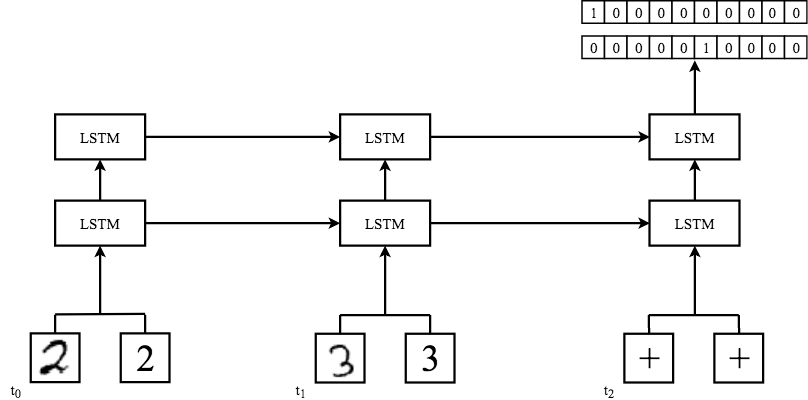
\includegraphics[max width=\textwidth]{sequential-model-with-symbols}
	\caption{A deep LSTM network that accepts a sequence of two operands and an operator each accompanied by a symbolic channel. The model learns to perform addition on the operands and produces an output in one-hot vector form.}
	\label{fig:sequential-model-with-symbols}
\end{figure}

Figure \ref{fig:sequential-model-with-symbols} shows an architecture that includes an explicit symbolic channel alongside the handwritten inputs. The network is composed of 1568 input units representing one 28x28 handwritten digit and another 28x28 image representing the clear symbol. The network outputs two one-hot vectors representing the sum of the inputs. Training is conducted by supplying sequences of three inputs; the two operands followed by the operator.

\paragraph{Implicit Symbols}

\begin{figure}[t]
	\centering
	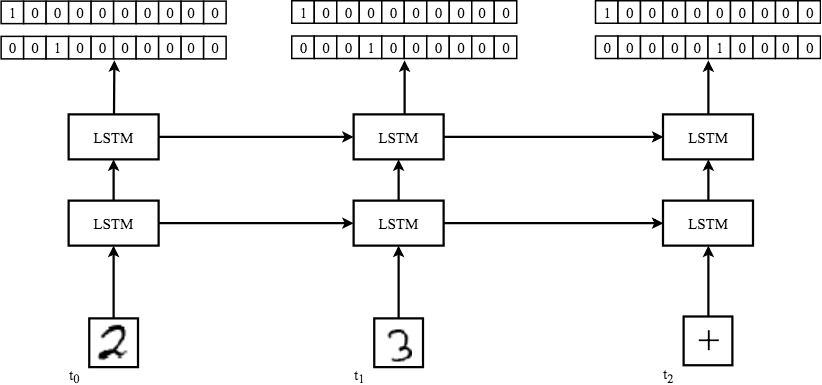
\includegraphics[max width=\textwidth]{sequential-model-with-classes}
	\caption{A deep LSTM network that accepts a sequence of two operands and an operator. The model learns to classify the operands before performing the addition when the operator is presented.}
	\label{fig:sequential-model-with-classes}
\end{figure}

Figure \ref{fig:sequential-model-with-classes} depicts an architecture that uses the second approach of implicit symbols. Here the network does not include a symbolic channel with the inputs. Instead, the network accepts 784 input units representing a 28x28 handwritten digit, one at a time. Each time a handwritten digit is provided, the model is trained to produce the value of that digit on the output channel. If an arithmetic operator is provided to the network, the model will output the result of the operation on the previous inputs. We believe that teaching the network to properly classify the inputs before performing the operation is similar to training the model using the clear symbolic inputs. The LSTM layers should be able to maintain the classes learned within their context, therefore, providing the same utility a symbolic channel would provide.

\bigskip

Symbols provide consistency that the neural network models can use to learn to perform the mathematical operations instead of relying solely on the noisy handwritten inputs. By successfully mapping the noisy inputs to the clear symbols, the job of the learning system becomes discovering a set of rules that accepts the clear symbols along with an operator to produce a result. Without the presence of these symbols, our neural networks would be susceptible to the high variation exhibited by the noisy inputs and therefore would need more training examples, making learning expensive.

We can explain the role of the symbol channel in terms of Bayesian inference. The probability of finding an optimum representation $h$ in the hypothesis space is affected by the presence of evidence, in our case, the classification data $C$ (symbols) and the noisy training data $D$. From Bayes' Theorem this can be given as:
\begin{equation}
p(h|C,D) = \frac{p(C,D|h) \cdot p(h)}{p(C,D)}
\end{equation}
The Maximum a posteriori hypothesis (assume prior hypotheses are equally likely, and data is common divisor) is given by:
\begin{equation}
h_{MAP} = \argmax_h p(C,D|h) p(h)
\end{equation}
However, $p(C,D|h) \cdot p(h)$ can be expressed as:
\begin{equation}
\begin{split}
p(C,D|h) \cdot p(h)\\
& = \frac{p(C,D,h)}{p(h)} \cdot p(h)\\
& = p(D | C, h) \cdot \frac{p(C, h)}{p(h)} \cdot p(h)\\
& = p(D | C, h) \cdot p(C |h) \cdot \frac{p(h)}{p(h)} \cdot p(h)\\
& = p(D | C, h) \cdot p(C |h) \cdot p(h)
\end{split}
\end{equation}
This means that the best hypothesis is the one that maximizes the product of the probability of the hypothesis, $p(h)$, the probability of the correct symbol given a hypothesis, $p(C |h)$, and the probability of the correct arithmetic operation given both the correct symbol and the hypothesis, $p(D | C, h)$\cite{wiki:Bayesian_inference}. Therefore, correctly mapping the noisy digits to the classes increases the likelihood that the learning system will discover a hypothesis that will maximize the posteriori probability. The next section further develops our approach by explaining empirical techniques that we can use to better understand the role of symbols.   